\documentclass[11pt,a4paper]{article}

% ---------- Packages ----------
\usepackage[margin=1in]{geometry}
\usepackage{times}
\usepackage[T1]{fontenc}
\usepackage{titlesec}
\usepackage{enumitem}
\usepackage{booktabs}
\usepackage{array}
\usepackage{xcolor}
\usepackage{hyperref}
\usepackage{tikz}
\usetikzlibrary{positioning,arrows.meta,shapes.geometric,fit,backgrounds}
\usepackage{fancyhdr}
\usepackage{longtable}
\usepackage{parskip}
\usepackage{graphicx}
\usepackage{caption}
\usepackage{tocloft}

\emergencystretch=3em
\tolerance=1200
\setcounter{tocdepth}{2}

% ---------- Colors ----------
\definecolor{navy}{RGB}{22,45,80}
\definecolor{steel}{RGB}{70,110,150}
\definecolor{lightgray}{RGB}{245,245,245}

% ---------- Section styling ----------
\titleformat{\section}
  {\normalfont\Large\bfseries\color{navy}}
  {\thesection}{0.6em}{}
\titleformat{\subsection}
  {\normalfont\large\bfseries\color{steel}}
  {\thesubsection}{0.6em}{}
\titleformat{\subsubsection}
  {\normalfont\normalsize\bfseries\color{steel}}
  {\thesubsubsection}{0.6em}{}

% ---------- Header/Footer ----------
\pagestyle{fancy}
\fancyhf{}
\renewcommand{\headrulewidth}{0.4pt}
\fancyhead[L]{\small CA1: Mini Project -- Proposal \& System Design (Phase 1)}
\fancyhead[R]{\small NLP Course}
\fancyfoot[C]{\thepage}

% ---------- Hyperref ----------
\hypersetup{
  colorlinks=true,
  linkcolor=steel,
  urlcolor=black,
  citecolor=steel,
  pdftitle={LinkedIn Job Posting Classification and Personalized Job Recommendation System -- CA1 Project Proposal},
  pdfauthor={Himnish Kumar R, Gracy Sweety T, Rakshitha V, Ashish UK}
}

\setlist[itemize]{topsep=2pt,itemsep=2pt,parsep=0pt}
\setlist[enumerate]{topsep=2pt,itemsep=2pt,parsep=0pt}

\renewcommand{\cftsecfont}{\color{navy}}
\renewcommand{\cftsecpagefont}{\color{navy}}

\begin{document}

% =========================================================
% TITLE PAGE
% =========================================================
\begin{titlepage}
\centering
\vspace*{1.0cm}

{\large CA1: Mini Project -- Project Proposal \& System Design (Phase 1)}\\[0.3cm]
{\large NLP Mini Project -- Team Proposal Report}\\[1.2cm]

\rule{\linewidth}{0.6pt}\\[0.4cm]
{\Huge\bfseries\color{navy} An Integrated Pipeline for Fraudulent Job \\[0.2cm] Filtering, Seniority Classification, and \\[0.2cm] Explainable Candidate-Job Matching}\\[0.5cm]
\rule{\linewidth}{0.6pt}\\[1.2cm]

{\large\itshape LinkedIn Job Posting Classification and\\ Personalized Job Recommendation System}\\[2cm]

\begin{tabular}{ll}
\toprule
\textbf{Team Member} & \textbf{Registration No.} \\
\midrule
Himnish Kumar R & 25MCAR0032 \\
Gracy Sweety T  & 25MCAR0031 \\
Rakshitha V     & 25MCAR0038 \\
Ashish UK       & 25MCAR0027 \\
\bottomrule
\end{tabular}

\vfill

{\large \today}

\end{titlepage}

\clearpage
\tableofcontents
\clearpage

% =========================================================
% 1. TITLE AND OBJECTIVE
% =========================================================
\section{Title and Objective}
\label{sec:objective}

\subsection*{Title}
An Integrated Pipeline for Fraudulent Job Filtering, Seniority Classification, and
Explainable Candidate-Job Matching -- proposed as a LinkedIn Job Posting Classification
and Personalized Job Recommendation System.

\subsection*{Objective}
The objective of this project is to design a system that (1) filters fraudulent job
postings before they propagate into downstream processes, (2) classifies genuine
postings by category and seniority level, and (3) recommends ranked, explainable job
matches to candidates based on r\'esum\'e-to-requirement similarity. This directly
addresses a gap identified in our literature survey (Section~\ref{sec:literature}),
where fraud filtering, classification, and recommendation are typically designed,
trained, and evaluated as three disconnected systems rather than a single coherent
pipeline. This report documents that design in full: the problem it addresses, the
literature that motivates it, the datasets it will draw on, the preprocessing and
modeling approach it proposes, and the team plan for delivering it.

\subsection*{Motivation}
Online recruitment has become the dominant channel through which job seekers discover
opportunities, but that scale brings two well-documented costs. First, the same openness
that makes large job boards useful also makes them a target for fraudulent postings --
listings designed to harvest personal information, extract fees, or simply inflate a
platform's apparent activity. Second, even among genuine postings, the sheer volume makes
manual browsing an increasingly poor way for a candidate to find roles that actually
match their skills and experience. Most existing systems address only one side of this
problem at a time: fraud-detection research rarely considers what happens downstream in
a recommendation pipeline, and recommendation research typically assumes an
already-clean posting pool. This project proposes to address both sides together, and to
treat the ordering between them -- filter first, then classify, then recommend -- as a
deliberate design decision rather than an afterthought.

% =========================================================
% 2. PROBLEM STATEMENT
% =========================================================
\section{Problem Statement}
\label{sec:problem}

Online professional networks such as LinkedIn host a continuously growing volume of job
postings spanning industries, roles, and experience levels. Two related challenges arise
for both platforms and job seekers:

\begin{enumerate}
    \item Accurately classifying job postings by \textbf{category}, \textbf{seniority},
    and \textbf{genuineness}, given the well-documented prevalence of fraudulent
    listings; and
    \item \textbf{Matching candidates} to the postings most relevant to their skills,
    experience, and preferences.
\end{enumerate}

Existing academic and applied work treats these as separate problems: fraud/genuineness
detection is studied independently of category or seniority classification, and
recommendation systems are built assuming an already-clean posting pool. In practice,
fraudulent postings that leak into a recommendation pipeline directly degrade
recommendation quality and erode user trust. This project proposes a single pipeline
that filters, classifies, and recommends in sequence, so that each downstream stage
operates only on postings that have already been validated by the stage before it.

\subsection*{Illustrative Scenario}
Consider a recent graduate searching for entry-level data-analytics roles on a large job
board. Without genuineness filtering, some fraction of the postings they encounter are
scams designed to harvest personal information rather than genuine openings -- a
candidate has no reliable way to tell the difference from the listing text alone.
Without seniority classification, postings mislabeled or unlabeled by the original
poster are effectively invisible to a seniority-based search filter, even when they are
genuinely relevant. Without explainable recommendation, even a technically accurate
match gives the candidate no way to judge whether the system considered their actual
skills or something else entirely. Each of this project's three modules addresses one
link in that chain; the system design in Section~\ref{sec:methodology} treats the chain
as a whole rather than three independent tools a candidate would need to use separately.

\subsection*{Scope of This Phase}
This report covers Phase~1 of the project: problem framing, literature review, dataset
selection, and system design. It proposes an approach and a plan; it does not report
model training results, evaluation metrics, or system performance, since implementation
and evaluation are the subject of the project's next phase. Where this report describes
a technique (a preprocessing step, a modeling choice), it describes what is planned and
why, not what has already been measured.

\subsection*{Success Criteria for This Phase}
Consistent with that scope, success for Phase~1 is defined by planning quality rather
than model performance: a clearly justified real-world problem (Section~\ref{sec:objective}),
a literature review that identifies a genuine, well-supported gap
(Section~\ref{sec:gap}), datasets that are relevant, adequately sized, and appropriately
sourced for each module (Section~\ref{sec:dataset}), preprocessing techniques that are
appropriate and clearly documented (Section~\ref{sec:preprocessing}), and a team plan
with clearly defined roles and a realistic timeline (Section~\ref{sec:team}). Model
accuracy targets are intentionally deferred to the project's next phase, where they can
be stated against actual training results rather than asserted in advance.

\subsection*{Deliverables for This Phase}
\label{sec:deliverables}
Consistent with the assignment brief for this phase, the deliverable is this Project
Proposal Report in PDF format, covering the five required sections (Title and
Objective, Problem Statement, Literature Context, Dataset Details, Methodology and
System Design) plus the team responsibilities and timeline documentation this rubric
also requires. No code, trained models, or evaluation results are included in this
deliverable, since implementation is scoped to the project's next phase. Each team
member's individual contribution to this proposal is recorded in
Section~\ref{sec:team}.

% =========================================================
% 3. LITERATURE CONTEXT
% =========================================================
\section{Literature Context}
\label{sec:literature}

\subsection{Job Posting Classification}
\label{sec:lit-classification}

Nasser and Alzaanin~\cite{nasser2020} evaluated five classical machine learning
classifiers -- Multinomial Naive Bayes, SVM, Decision Tree, KNN, and Random Forest -- for
separating genuine and fraudulent job postings using TF-IDF text features on the EMSCAD
dataset, establishing a widely-cited baseline for classical-ML approaches to this task.
A follow-up genuineness-classification study~\cite{ijraset2021} applied Random Forest
with an oversampling strategy to correct class imbalance in real-vs-fake postings on the
same dataset, reporting accuracy above 98\%. Both studies work from the same underlying
premise that motivates our own Dataset choice for this sub-problem (Section~\ref{sec:dataset-emscad}):
that TF-IDF text representations, paired with classical ML classifiers and an explicit
strategy for class imbalance, are a strong and reproducible starting point for
fraud/genuineness detection.

More recent work reframes job-posting analysis as multi-class metadata extraction rather
than binary fraud detection~\cite{metadata2023}, using transformer embeddings (BERT/USE4)
and LLM-generated synthetic data to offset limited labeled-data availability. This
signals a plausible extension path beyond the classical baselines: once a classical
pipeline is working and evaluated, a transformer-based variant is a natural next
comparison point, and this project's design (Section~\ref{sec:methodology}) leaves room
for that extension explicitly. Large-scale labour-market-intelligence research~\cite{boselli}
has applied ML classification to job vacancies with an emphasis on multi-language,
standardized taxonomies rather than proprietary single-language category systems,
enabling broader real-time market monitoring -- a design consideration worth noting
given that this project's chosen LinkedIn dataset (Section~\ref{sec:dataset-linkedin})
uses its own internal skill and industry taxonomy, whose granularity we examine closely
during dataset planning.

\subsection{Preprocessing and Feature Extraction Approaches in Prior Work}
\label{sec:lit-preprocessing}

Since this proposal's own preprocessing plan (Section~\ref{sec:preprocessing}) draws
directly on established practice, it is worth reviewing what the surveyed literature
actually does at the feature-extraction stage rather than only at the modeling stage.
The classical fraud-classification baselines~\cite{nasser2020,ijraset2021} both rely on
TF-IDF vectorization over cleaned, lowercased, stopword-filtered text -- a comparatively
lightweight pipeline chosen specifically so that the modeling comparison (Naive Bayes vs.
SVM vs.\ Random Forest) is not confounded by an elaborate feature-engineering step. The
more recent metadata-extraction work~\cite{metadata2023} moves to transformer embeddings
(BERT, Universal Sentence Encoder) precisely because TF-IDF's bag-of-words assumption
discards word order and struggles with synonymy -- e.g.\ ``machine learning engineer''
and ``ML engineer'' produce near-orthogonal TF-IDF vectors despite being near-synonymous
job titles. This tradeoff is directly relevant to our own plan: TF-IDF is proposed as the
baseline representation for reproducibility and interpretability, with a transformer
embedding representation planned as a direct comparison once the baseline is validated,
rather than choosing one representation permanently at the proposal stage.

On the recommendation side, DSSM-style approaches~\cite{mishra2022} similarly move past
raw keyword matching toward learned semantic representations, and the hybrid-filtering
literature~\cite{hybrid} combines content-based similarity (which needs a good text
representation) with collaborative signals (which this project's datasets do not
directly support, since we do not have historical candidate-application interaction
data). This is a scoping decision worth stating plainly: this project's recommendation
module is planned as content-based, not collaborative, because the available dataset
(Section~\ref{sec:dataset-resume}) supports the former and not the latter.

\subsection{Class Imbalance Handling in Prior Work}
\label{sec:lit-imbalance}

Class imbalance is a recurring theme across the fraud-detection literature specifically,
since fraudulent postings are a small minority of any real posting pool by construction.
The Random-Forest-with-oversampling study~\cite{ijraset2021} addresses this directly, and
its reported accuracy above 98\% is a useful benchmark for our own planned EMSCAD
baseline. More broadly, oversampling (SMOTE and its variants), class-weighting, and
threshold adjustment are the three standard approaches to this problem in the
classification literature; this proposal's plan (Section~\ref{sec:preprocessing}) opts
for SMOTE specifically for the binary, more strongly imbalanced Module~1 problem, and
class-weighting for the six-class, less extremely imbalanced Module~2 problem, on the
reasoning that SMOTE's synthetic-sample generation is more justified when the minority
class is a very small fraction of the data, while class-weighting is a cheaper and
sufficient correction when the imbalance, though real, is less severe.

Mishra and Rathi~\cite{mishra2022} proposed an enhanced Deep Semantic Structured Model
(DSSM) to improve semantic matching between r\'esum\'es and job descriptions beyond
earlier keyword-based techniques. Deep reinforcement learning has also been applied to
job recommendation~\cite{drl}, using historical user-profile and job-description data to
outperform traditional recommendation baselines in experimental evaluation. Hybrid
filtering -- combining collaborative and content-based approaches -- has been used to
improve precision, recall, and F1 in systems that recommend careers based on candidate
skills and interests~\cite{hybrid}.

Personality-aware matching approaches~\cite{jobfit} extend recommendation beyond
hard-skill overlap, integrating trait-based assessments with LLM-processed job
descriptions to account for career fit and retention, not just qualification match.
CareerCue~\cite{careercue} proposes a modular pipeline that parses LinkedIn profile data
for skills and experience, fetches live postings via a job-aggregation API, and produces
ranked, explainable recommendations -- while explicitly noting platform dependency,
limited personalization, and data-privacy concerns as unresolved issues. A broader review
of ML-based job recommendation systems~\cite{review2025} documents the shift toward
hybrid recommendation models and highlights fairness and debiasing in ranking as an
active research concern. Taken together, this thread of literature converges on
semantic, content-based matching (as opposed to pure keyword overlap) as the current
state of the art, and on explainability as a persistently under-addressed requirement --
both of which directly shape the recommendation module's design in
Section~\ref{sec:module3-design}.

\subsection{Existing Solution Analysis}
\label{sec:lit-existing}

LinkedIn's own platform already performs large-scale job matching (its ``Jobs for You''
feed), but the underlying ranking models and signals are proprietary and closed to
academic study -- leaving room for an independent, transparent system built on public
job-posting data. Academic prototypes such as r\'esum\'e-based company recommenders
demonstrate the feasibility of a r\'esum\'e $\rightarrow$ feature extraction
$\rightarrow$ classifier/recommender pipeline (KNN, SVM, Random Forest), but are
typically validated on small, single-institution datasets rather than a real job board's
actual posting corpus. CareerCue-style systems show that a profile extractor plus job
fetcher plus scoring/notification layer is achievable with lightweight tooling, but
generally rely on rule-based scoring rather than transformer-based semantic matching, and
are rarely benchmarked against classical ML baselines.

\begin{table}[h]
\centering
\small
\begin{tabular}{@{}p{3.6cm}p{5.6cm}p{5.4cm}@{}}
\toprule
\textbf{Approach} & \textbf{Strength} & \textbf{Limitation relative to this proposal} \\
\midrule
LinkedIn ``Jobs for You'' & Massive scale, real user engagement signal & Proprietary,
not reproducible or auditable \\
Classical fraud classifiers~\cite{nasser2020,ijraset2021} & Strong, reproducible
accuracy on EMSCAD & Evaluated in isolation from recommendation \\
DSSM / RL recommenders~\cite{mishra2022,drl} & Semantic matching beyond keyword overlap
& No fraud-filtering stage upstream \\
CareerCue~\cite{careercue} & End-to-end profile-to-recommendation pipeline & Rule-based
scoring, limited explainability \\
\bottomrule
\end{tabular}
\caption{Summary comparison of surveyed approaches against this project's proposed scope.}
\label{tab:lit-comparison}
\end{table}

Across the systems surveyed, two gaps recur, summarized in Table~\ref{tab:lit-comparison}.
First, job-posting genuineness/fraud filtering and job recommendation are almost always
treated as separate problems, despite fraudulent postings directly degrading
recommendation quality when left unfiltered. Second, explainability is inconsistently
addressed -- most systems return a ranked list without surfacing why a job was matched,
which limits user trust, as noted explicitly in the CareerCue evaluation.

\subsection{Identified Gap and Justification}
\label{sec:gap}

The reviewed literature treats classification (category/seniority/genuineness) and
recommendation (candidate-job matching) as largely independent problems, each with
mature but separate baselines. A combined pipeline -- filtering and categorizing
postings before they enter a hybrid, explainable recommendation stage -- addresses gaps
common to both threads: fraudulent-listing leakage into recommendations, weak
explainability, and limited handling of cold-start users or newly posted jobs. This is
the specific contribution this project proposes to make: not a new classification or
recommendation algorithm in isolation, but a system-level integration that the surveyed
literature does not attempt.

% =========================================================
% 4. DATASET DETAILS
% =========================================================
\section{Dataset Details}
\label{sec:dataset}

The project will draw on three complementary, publicly available datasets, one per
pipeline stage. All three have been identified and reviewed during this proposal phase;
collection and preprocessing are planned for the project's next phase.

\subsection{LinkedIn Job Postings (2023--2024) --- Category/Seniority Classification}
\label{sec:dataset-linkedin}

\textbf{Source:} Kaggle, dataset \textit{arshkon/linkedin-job-postings}. 123{,}849 real
LinkedIn postings scraped across industries and locations, split across 11 files: a core
\texttt{postings} table plus normalized \texttt{skills}, \texttt{industries},
\texttt{benefits}, and \texttt{salaries} tables keyed by \texttt{job\_id}, and
\texttt{companies} metadata.

\begin{center}
\small
\begin{tabular}{@{}p{4.6cm}p{1.6cm}p{7cm}@{}}
\toprule
\textbf{File} & \textbf{Rows} & \textbf{Purpose} \\
\midrule
\url{postings.csv} & 123{,}849 & Core table: title, description, location, salary
fields, \texttt{formatted\_experience\_level}, work type \\[2pt]
\url{jobs/job_skills.csv} & 213{,}768 & job\_id $\to$ skill\_abr (many-to-many) \\[2pt]
\url{jobs/job_industries.csv} & 164{,}808 & job\_id $\to$ industry\_id \\[2pt]
\url{jobs/benefits.csv} & 67{,}943 & job\_id $\to$ benefit type \\[2pt]
\url{jobs/salaries.csv} & 40{,}785 & Normalized salary records \\[2pt]
\url{mappings/skills.csv} & 35 & skill\_abr $\to$ skill\_name \\[2pt]
\url{mappings/industries.csv} & 422 & industry\_id $\to$ industry\_name \\[2pt]
\url{companies/companies.csv} & 24{,}473 & company\_id $\to$ name, size, location \\
\bottomrule
\end{tabular}
\end{center}
\normalsize

\textbf{Planned classification target:} \texttt{formatted\_experience\_level} -- six
classes (Entry, Associate, Mid-Senior, Director, Executive, Internship). Initial
exploration shows this field populated for roughly three-quarters of postings, with the
remainder forming a pool the trained model would need to label at inference time rather
than discard -- a design requirement carried into Section~\ref{sec:module2-design}.
\textbf{Anticipated data-quality considerations:} salary fields appear sparsely
populated across the dataset and are not planned as a primary feature for this reason.
The skills/industries mapping tables use LinkedIn's own internal taxonomy rather than a
free-form skill vocabulary -- notably, the skills mapping table has only 35 entries
total, which initial review flags as a possible granularity concern worth close
attention during preprocessing (Section~\ref{sec:preprocessing}), since an overly coarse
taxonomy would limit its usefulness for fine-grained matching in Module~3.

\subsection{EMSCAD --- Genuineness/Fraud Classification}
\label{sec:dataset-emscad}

\textbf{Source:} Kaggle, dataset \textit{shivamb/real-or-fake-fake-jobposting-prediction}
(Employment Scam Aegean Dataset). 17{,}880 job postings published 2012--2014, of which
866 (4.8\%) are manually annotated as fraudulent -- the same dataset used by the
classical-ML baselines in Section~\ref{sec:lit-classification}, which will let our
planned reproduction be compared directly against published results.

\textbf{Fields:} title, location, department, salary\_range, company\_profile,
description, requirements, benefits, telecommuting, has\_company\_logo, has\_questions,
employment\_type, required\_experience, required\_education, industry, function,
\texttt{fraudulent} (target). \textbf{Anticipated data-quality considerations:} the
dataset is strongly imbalanced (17{,}014 genuine vs.\ 866 fraudulent postings), which the
methodology plan (Section~\ref{sec:module1-design}) addresses with SMOTE oversampling
applied only to a training split, to avoid inflating any future evaluation with
synthetic samples.

\subsection{R\'esum\'e--Job Matching Dataset --- Recommendation Module}
\label{sec:dataset-resume}

\textbf{Source:} Kaggle r\'esum\'e-parsing/job-matching dataset. 9{,}544 paired records,
each combining a candidate r\'esum\'e (career objective, skills, education, work
history, certifications) with a target job's requirements (position, required
education, required experience, required skills) and a pre-computed \texttt{matched\_score}.

This is the key asset for Module~3: it supplies \emph{ground-truth} match scores, so the
recommendation component can be trained as a supervised ranking/regression task rather
than relying purely on unsupervised similarity heuristics, which is a step beyond most of
the surveyed recommendation literature. \textbf{Anticipated data-quality considerations:}
initial inspection shows that structurally similar fields are serialized differently
across columns (list-formatted vs.\ plain delimited text), which the preprocessing plan
treats as a parsing requirement rather than something to defer.

\subsection{Dataset Summary}

Table~\ref{tab:dataset-summary} summarizes all three datasets against the pipeline stage
they will support.

\begin{table}[h]
\centering
\small
\begin{tabular}{@{}p{3.2cm}p{1.9cm}p{3.6cm}p{5.2cm}@{}}
\toprule
\textbf{Dataset} & \textbf{Size} & \textbf{Target Module} & \textbf{Prediction Target} \\
\midrule
LinkedIn Job Postings & 123{,}849 rows & Module 2 (Category/Seniority) &
\texttt{formatted\_experience\_level} (6 classes) \\
EMSCAD & 17{,}880 rows & Module 1 (Genuineness) & \texttt{fraudulent} (binary) \\
R\'esum\'e--Job Matching & 9{,}544 pairs & Module 3 (Recommendation) &
\texttt{matched\_score} (continuous) \\
\bottomrule
\end{tabular}
\caption{Summary of the three datasets proposed for this project, one per module.}
\label{tab:dataset-summary}
\end{table}

% =========================================================
% 5. METHODOLOGY AND SYSTEM DESIGN
% =========================================================
\section{Methodology and System Design}
\label{sec:methodology}

\subsection{Design Rationale}

The system is proposed as three modules wired into a single sequential pipeline
(Figure~\ref{fig:architecture}). Postings would first pass through the genuineness
filter (Module~1); only postings scored genuine would be labeled by the
category/seniority classifier (Module~2) and become eligible to enter the
candidate-matching pool (Module~3). This ordering -- filter, then classify, then
recommend -- is the project's central architectural decision, directly motivated by the
literature gap identified in Section~\ref{sec:gap}: fraudulent postings should never
reach a recommendation stage undetected. Each module is designed to be trained and
validated independently first, so that its own performance can be measured cleanly
before the modules are combined -- and only then evaluated together as an integrated
system, since a module's in-isolation performance is not automatically evidence that it
will behave well once wired into the full pipeline.

\begin{figure}[h]
\centering
\resizebox{\textwidth}{!}{%
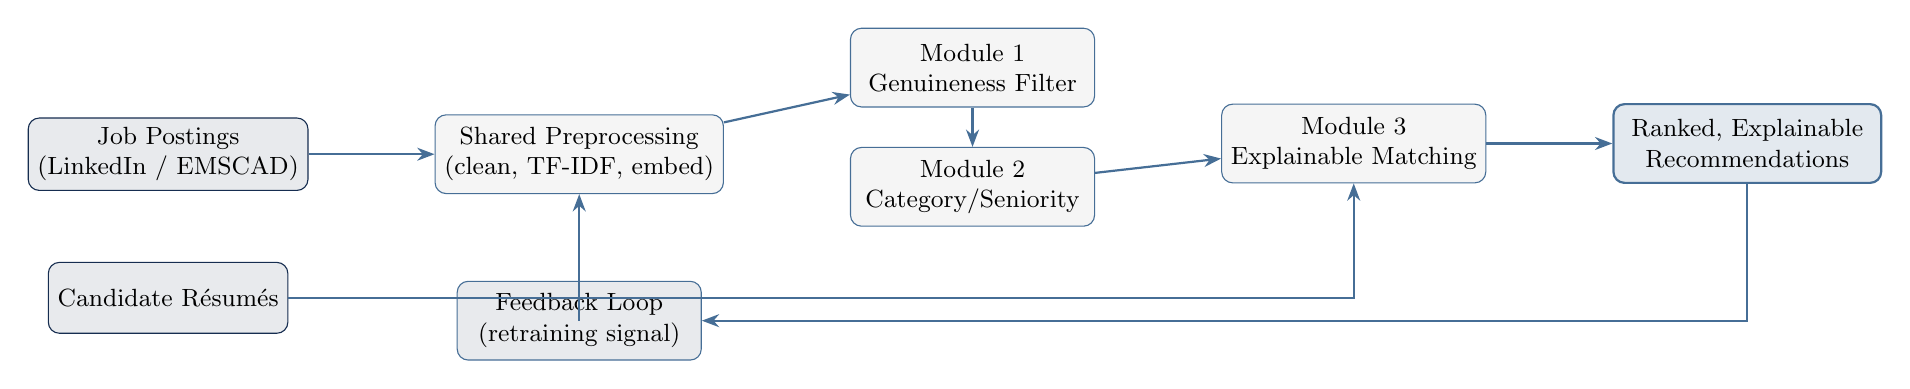
\begin{tikzpicture}[
  node distance=0.9cm and 1.3cm,
  box/.style={draw, rounded corners, minimum width=3.1cm, minimum height=1cm, align=center, font=\small, fill=lightgray, draw=steel},
  input/.style={draw, rounded corners, minimum width=2.6cm, minimum height=0.9cm, align=center, font=\small, fill=navy!10, draw=navy},
  output/.style={draw, rounded corners, minimum width=3.4cm, minimum height=1cm, align=center, font=\small, fill=steel!15, draw=steel, thick},
  arr/.style={-{Stealth[length=2.2mm]}, thick, steel}
]

\node[input] (jobs) {Job Postings\\(LinkedIn / EMSCAD)};
\node[input, below=of jobs] (resumes) {Candidate R\'esum\'es};

\node[box, right=1.6cm of jobs] (prep) {Shared Preprocessing\\(clean, TF-IDF, embed)};

\node[box, right=1.6cm of prep, yshift=1.1cm] (m1) {Module 1\\Genuineness Filter};
\node[box, below=0.5cm of m1] (m2) {Module 2\\Category/Seniority};

\node[box, right=1.6cm of m2, yshift=0.55cm] (m3) {Module 3\\Explainable Matching};

\node[output, right=1.6cm of m3] (out) {Ranked, Explainable\\Recommendations};

\node[box, below=1.1cm of prep, fill=navy!10] (fb) {Feedback Loop\\(retraining signal)};

\draw[arr] (jobs) -- (prep);
\draw[arr] (prep) -- (m1);
\draw[arr] (m1) -- (m2);
\draw[arr] (m2) -- (m3);
\draw[arr] (resumes) -| (m3);
\draw[arr] (m3) -- (out);
\draw[arr] (out) |- (fb);
\draw[arr] (fb) -| (prep);

\end{tikzpicture}%
}
\caption{Proposed system architecture: sequential fraud filtering and classification gate
the pool of postings eligible for explainable candidate matching, with a feedback loop
for continuous retraining.}
\label{fig:architecture}
\end{figure}

\subsection{Data Preprocessing Plan}
\label{sec:preprocessing}

Preprocessing is planned as a shared pipeline applied consistently across all three
datasets' free-text fields (\texttt{description}, \texttt{career\_objective},
\texttt{responsibilities}, \texttt{requirements}), so that no module's text
representation is built with different assumptions than the others':

\begin{itemize}
    \item \textbf{Lowercasing and noise removal:} all text lowercased; HTML tags and
    URLs stripped via pattern matching, since several source fields (job descriptions in
    particular) are known to contain markup artifacts from web scraping.
    \item \textbf{Tokenization:} whitespace/regex-based tokenization after
    non-alphabetic character removal, chosen over a heavier subword tokenizer at this
    stage to keep the classical-ML baselines (Section~\ref{sec:lit-classification})
    directly comparable to their published counterparts.
    \item \textbf{Stopword removal:} standard English stopword list, to reduce
    dimensionality in the resulting TF-IDF representation without discarding
    domain-relevant terms.
    \item \textbf{Normalization:} lemmatization rather than stemming, to keep cleaned
    tokens as recognizable dictionary words -- relevant later for the explainability
    goal in Module~3, where surfaced feature importances need to be human-readable.
    \item \textbf{Structured/categorical fields:} binary flags (e.g.\
    \texttt{telecommuting}, \texttt{has\_company\_logo}) planned as direct numeric
    features alongside the text representation, rather than being discarded or
    text-encoded, since the literature identifies them as informative signals in their
    own right.
    \item \textbf{Class imbalance:} SMOTE oversampling planned for Module~1's training
    split specifically, given EMSCAD's 4.8\% fraud rate; Module~2's six-class imbalance
    is planned to be handled via class-weighted loss instead, since oversampling at that
    dataset's row count and feature dimensionality would be considerably more expensive.
    \item \textbf{Feature extraction:} TF-IDF representations (planned at 5{,}000
    features, unigrams and bigrams) as the primary text representation across all three
    modules, consistent with the classical baselines reviewed in
    Section~\ref{sec:literature}, with a transformer-embedding representation
    (e.g.\ SBERT-style sentence embeddings) planned as a comparison point once the
    classical pipeline is working end-to-end.
\end{itemize}

\subsection{Module 1 --- Genuineness Classification (Planned Approach)}
\label{sec:module1-design}

Trained on EMSCAD. Baseline plan: TF-IDF features (title, description, requirements)
combined with the three structured binary flags described in
Section~\ref{sec:preprocessing}, evaluated across Naive Bayes, SVM, and Random Forest
classifiers, with SMOTE applied to the training split to address the 4.8\% fraud rate,
directly replicating the methodology of~\cite{nasser2020,ijraset2021} as a baseline
before any extension. These three classifiers are planned specifically because they
span a useful range of modeling assumptions: Naive Bayes as a fast, strongly-regularized
baseline that assumes feature independence; linear SVM as a margin-based classifier
well-suited to high-dimensional sparse TF-IDF input; and Random Forest as a non-linear
ensemble capable of capturing feature interactions neither of the other two can. Training
all three and comparing them empirically is preferred over committing to one in advance,
since the literature itself does not agree on a single best classifier for this task.
\textbf{Planned output:} a binary genuineness score attached to
every posting, which becomes the gating signal for Module~2.

\subsection{Module 2 --- Category/Seniority Classification (Planned Approach)}
\label{sec:module2-design}

Trained on the LinkedIn Postings dataset. Planned as a multi-class classifier predicting
\texttt{formatted\_experience\_level} from title, description, and mapped
skills/industries, using the same TF-IDF representation strategy as Module~1 for
consistency. Class-weighted classical classifiers (Logistic Regression, SVM, Random
Forest) are planned as the baseline comparison set, again chosen to compare a
linear-probabilistic model, a margin-based model, and a non-linear ensemble against each
other rather than assuming in advance which style of classifier suits a six-class,
imbalanced target best. Postings without a ground-truth
label are planned to be scored by the trained model at inference time rather than
discarded, since roughly a quarter of the dataset falls into this category and discarding
it would meaningfully shrink the usable posting pool for downstream recommendation.

\subsection{Module 3 --- Recommendation Engine (Planned Approach)}
\label{sec:module3-design}

Trained on the r\'esum\'e--job matching dataset. Planned features are the semantic
similarity between candidate-side text (skills, career objective, responsibilities) and
job-side text (required skills, education, experience), trained against the
\texttt{matched\_score} ground truth as a supervised regression target rather than an
unsupervised similarity heuristic -- a deliberate choice, since an unsupervised
similarity score alone would have no way to be calibrated against this dataset's actual
notion of a good match, whereas a supervised model can learn that calibration directly
from the provided ground truth. Feature-level contributions (e.g.\ which skills or
education fields drove a given score) are planned to be surfaced alongside each
recommendation, directly addressing the explainability gap identified in
Section~\ref{sec:lit-existing}. Both a small set of named, interpretable similarity
features and a higher-capacity representation are planned to be compared once training
begins, so that the accuracy/explainability tradeoff this problem presents is decided
with evidence rather than assumed in either direction at the proposal stage.

\subsection{Evaluation Plan}
\label{sec:evaluation-plan}

Each module is planned to be evaluated with metrics matched to its task, on a held-out
test split never seen during training or preprocessing-parameter selection:

\begin{itemize}
    \item \textbf{Module~1 (Genuineness):} accuracy, precision/recall/F1 on the fraud
    class specifically (not just overall accuracy, since the class imbalance described
    in Section~\ref{sec:dataset-emscad} makes overall accuracy a poor standalone signal),
    and ROC-AUC. Confusion matrices are planned to be reported alongside summary metrics
    so that the precision/recall tradeoff for each candidate classifier is visible, not
    just a single blended score.
    \item \textbf{Module~2 (Category/Seniority):} accuracy, macro-F1, and weighted-F1
    across all six classes, with macro-F1 planned as the primary model-selection metric
    specifically because accuracy alone would reward a model for the dominant classes
    (Mid-Senior, Entry) while masking poor performance on rare classes (Executive,
    Internship).
    \item \textbf{Module~3 (Recommendation):} mean absolute error (MAE), root mean
    squared error (RMSE), and R\textsuperscript{2} against the \texttt{matched\_score}
    target, since this is planned as a regression task rather than a classification one.
    \item \textbf{Integrated pipeline:} beyond each module's own metrics, the
    integration plan (Section~\ref{sec:integration}) calls for inspecting a sample of
    end-to-end recommendations qualitatively -- checking whether top-ranked results are
    topically sensible for a given candidate profile -- since a strong module-level
    metric does not by itself guarantee that the combined system produces sensible
    output once modules are chained together.
\end{itemize}

For every module, multiple candidate algorithms (at minimum two, per this phase's
requirements) are planned to be trained and compared side by side rather than
committing to a single algorithm in advance, so that model selection is evidence-based
once training is underway.

\subsection{Integration Plan}
\label{sec:integration}

Once each module is independently trained and validated, the fusion plan is to route a
sample of postings through the full sequence shown in Figure~\ref{fig:architecture}:
Module~1 filters, Module~2 labels the survivors, and Module~3 ranks them against a
candidate profile with an explanation attached to each ranked result. This integrated
run is planned as a distinct evaluation step from each module's individual validation,
on the view that a module's standalone metrics are not sufficient evidence that the
combined system will behave as designed -- a risk this proposal treats as worth planning
for explicitly rather than assuming away.

% =========================================================
% 6. RISK ASSESSMENT AND MITIGATION STRATEGY
% =========================================================
\section{Risk Assessment and Mitigation Strategy}
\label{sec:risk}

A proposal that only describes what is expected to work is less useful than one that
also names what could go wrong. Table~\ref{tab:risks} sets out the risks this team has
identified during planning, alongside the mitigation each risk motivates in the design
already described in Section~\ref{sec:methodology}.

\begin{table}[h]
\centering
\small
\begin{tabular}{@{}p{4.4cm}p{2.6cm}p{6.2cm}@{}}
\toprule
\textbf{Risk} & \textbf{Likelihood} & \textbf{Planned Mitigation} \\
\midrule
Severe class imbalance in EMSCAD (4.8\% fraud) degrades Module~1 recall & High & SMOTE
oversampling on the training split only (Section~\ref{sec:preprocessing}); evaluation
plan reports precision/recall/F1 on the fraud class specifically, not just accuracy
(Section~\ref{sec:evaluation-plan}) \\[4pt]
LinkedIn's skill taxonomy (35 categories) is too coarse for fine-grained matching in
Module~3 & Medium-High & Flagged explicitly during dataset review
(Section~\ref{sec:dataset-linkedin}); free-text description fields planned as a fallback
signal alongside the mapped taxonomy \\[4pt]
Models trained on one dataset (e.g.\ the r\'esum\'e--job matching corpus) may not
generalize when applied within a pipeline populated by a different dataset's postings
(LinkedIn) & Medium-High & Integration plan (Section~\ref{sec:integration}) treats
end-to-end pipeline evaluation as a distinct, required step rather than assuming
module-level metrics transfer automatically \\[4pt]
24\% of LinkedIn postings lack a ground-truth seniority label & Certain (known from
initial exploration) & Design requirement to score unlabeled postings at inference
rather than discard them (Section~\ref{sec:module2-design}) \\[4pt]
Heterogeneous data formats across datasets (e.g.\ list-encoded vs.\ plain-text fields)
slow down preprocessing & Medium & Identified during dataset review
(Section~\ref{sec:dataset-resume}) and scheduled explicitly in the project timeline
(Table~\ref{tab:timeline}) rather than left as an unplanned blocker \\
\bottomrule
\end{tabular}
\caption{Risks identified during proposal planning and their corresponding mitigations.}
\label{tab:risks}
\end{table}

The risk most worth naming explicitly is the third: this project's own architecture
(Figure~\ref{fig:architecture}) trains three modules on three different datasets and
then combines them into one pipeline. Nothing about training each module well
guarantees that its behavior transfers cleanly once it is applied to a different data
source within the combined system. This is precisely why the integration plan
(Section~\ref{sec:integration}) is scoped as a required, separate evaluation step rather
than an optional final check.

% =========================================================
% 7. ETHICAL CONSIDERATIONS AND DATA PRIVACY
% =========================================================
\section{Ethical Considerations and Data Privacy}
\label{sec:ethics}

\subsection{Data Provenance and Licensing}

All three datasets (Sections~\ref{sec:dataset-linkedin}--\ref{sec:dataset-resume}) are
publicly available on Kaggle under their respective dataset licenses. No new personal
data collection is planned; all candidate and posting data used is pre-existing,
de-identified at the level provided by the original dataset publishers. The project
plans to use these datasets strictly for academic, non-commercial coursework, consistent
with their stated terms.

\subsection{Bias and Fairness}

Both classification modules (genuineness and seniority) carry a fairness risk worth
naming at the design stage rather than discovering after training: a model trained on
historical postings can learn and reproduce whatever biases are already present in that
historical data -- for example, if certain job categories or phrasings are
disproportionately associated with the fraud label in EMSCAD for reasons unrelated to
actual fraud risk, a classifier could learn a spurious shortcut rather than a genuine
signal. The evaluation plan (Section~\ref{sec:evaluation-plan}) reports per-class metrics
(not just aggregate accuracy) specifically so that uneven performance across classes --
a symptom of exactly this kind of learned bias -- would be visible rather than averaged
away.

\subsection{Explainability as an Ethical Requirement, Not Only a Technical One}

This project's emphasis on explainable recommendations (Section~\ref{sec:module3-design})
is motivated by more than usability. A candidate who is shown a job recommendation with
no rationale has no way to assess whether the system is matching them on relevant
qualifications or on some other, potentially inappropriate signal. Surfacing which
specific skills or requirements drove a match is planned as a way to make that
assessment possible for the end user, not only as a debugging aid for the development
team.

\subsection{Limitations of This Section}

This proposal is a coursework project evaluated on a fixed academic timeline
(Table~\ref{tab:timeline}), using historical, de-identified public datasets rather than
live user data. A production deployment of a system like this would need considerably
more rigorous fairness auditing, ongoing bias monitoring, and explicit user consent
mechanisms than this project's scope allows; this section names the considerations
relevant at proposal stage, not a complete responsible-deployment plan.

% =========================================================
% 8. TEAM RESPONSIBILITIES AND PROJECT TIMELINE
% =========================================================
\section{Team Responsibilities and Project Timeline}
\label{sec:team}

\subsection{Team Responsibilities}

\begin{center}
\begin{tabular}{@{}p{3.6cm}p{3cm}p{7cm}@{}}
\toprule
\textbf{Team Member} & \textbf{Reg. No.} & \textbf{Primary Responsibility} \\
\midrule
Himnish Kumar R & 25MCAR0032 & System design and architecture; overall pipeline
design (Figure~\ref{fig:architecture}); Module~1 and Module~2 methodology planning \\
Gracy Sweety T & 25MCAR0031 & Dataset identification and validation across all three
sources; documentation \\
Rakshitha V & 25MCAR0038 & Data preprocessing pipeline design (text cleaning,
TF-IDF/embedding strategy) \\
Ashish UK & 25MCAR0027 & Module~3 methodology planning; report compilation and
literature review \\
\bottomrule
\end{tabular}
\end{center}

\textit{Note: this allocation reflects primary ownership for planning purposes; all
members contribute to review and documentation across sections.}

\subsection{Collaboration Plan}

The team plans weekly check-ins aligned with the milestones in
Table~\ref{tab:timeline}, so that dependencies between roles are surfaced early -- for
example, Module~2's design (owned by Himnish Kumar R) depends on the LinkedIn dataset's
skill-taxonomy granularity assessment (owned by Gracy Sweety T), and both need to be
resolved before Module~3's design (owned by Ashish UK) can finalize its planned
candidate-side feature set. Shared documentation is planned to be maintained
continuously through the phase rather than assembled only at submission time, so that
this report reflects work actually completed at each milestone rather than a
retrospective reconstruction.

\subsection{Project Timeline}

Table~\ref{tab:timeline} sets out the planned schedule for this phase of the project,
from initial problem selection through proposal submission.

\begin{table}[h]
\centering
\begin{tabular}{@{}p{2.2cm}p{5.2cm}p{5.4cm}@{}}
\toprule
\textbf{Week} & \textbf{Milestone} & \textbf{Primary Owner(s)} \\
\midrule
Week 1 & Problem ideation, real-world NLP problem selection, faculty consultation and
approval & Full team \\
Week 2 & Dataset identification and shortlisting across candidate sources (Kaggle
searches for fraud-detection, job-classification, and r\'esum\'e-matching datasets) &
Gracy Sweety T \\
Week 3 & Literature review -- collecting and synthesizing papers on job posting
classification and personalized recommendation & Ashish UK, with review from full team \\
Week 4 & Dataset validation (schema review, size/quality checks per dataset) and
preprocessing pipeline design & Rakshitha V \\
Week 5 & System architecture design, module-by-module methodology planning, and
integration plan & Himnish Kumar R \\
Week 6 & Proposal report drafting, internal review, and submission & Full team \\
\bottomrule
\end{tabular}
\caption{Planned six-week timeline for Phase 1 (proposal and system design).}
\label{tab:timeline}
\end{table}

This timeline is scoped to Phase~1 activities only -- problem framing, dataset
selection, and system design -- consistent with this report's stated scope
(Section~\ref{sec:problem}). Implementation, model training, and evaluation are planned
for the project's next phase and are outside this timeline's scope.

% =========================================================
% GLOSSARY
% =========================================================
\section*{Glossary of Key Terms}
\addcontentsline{toc}{section}{Glossary of Key Terms}

\begin{description}[leftmargin=3.2cm, style=nextline]
\item[TF-IDF] Term Frequency-Inverse Document Frequency: a text representation that
weights each word in a document by how frequent it is locally versus how common it is
across the whole corpus, giving higher weight to distinctive terms.
\item[SMOTE] Synthetic Minority Oversampling Technique: a method for addressing class
imbalance by generating synthetic examples of the minority class rather than simply
duplicating existing ones.
\item[Class-weighted loss] A training adjustment that penalizes misclassifying a rare
class more heavily than a common one, without generating any synthetic data.
\item[Macro-F1] The F1 score (harmonic mean of precision and recall) averaged equally
across all classes, regardless of how many examples each class has -- as opposed to
weighted-F1, which weights each class by its frequency.
\item[R\textsuperscript{2} (coefficient of determination)] A regression metric
measuring the proportion of variance in the target variable explained by a model's
predictions; ranges up to 1.0, with higher values indicating a better fit.
\item[Genuineness classification] This project's term for the binary task of labeling a
job posting as legitimate or fraudulent.
\item[Cold-start problem] The general recommendation-systems challenge of producing
useful recommendations for a new user or item with little to no historical interaction
data available.
\item[Explainability] The property of a model's output being accompanied by a
human-interpretable rationale for why that output was produced, as opposed to a bare
score or ranking with no accompanying justification.
\item[Content-based recommendation] A recommendation approach that ranks items by
similarity between item content (e.g.\ job requirements) and user content (e.g.\
r\'esum\'e text), as opposed to collaborative filtering, which relies on patterns across
many users' historical interactions.
\end{description}

% =========================================================
% REFERENCES
% =========================================================
\clearpage
\addcontentsline{toc}{section}{References}
\begin{thebibliography}{99}

\bibitem{nasser2020} Nasser, I., \& Alzaanin, A.~H. (2020). Machine Learning and Job Posting Classification: A Comparative Study. \textit{International Journal of Engineering and Information Systems (IJEAIS)}, 4(9), 6--14.

\bibitem{ijraset2021} Classification of Genuinity in Job Posting Using Machine Learning. \textit{International Journal for Research in Applied Science \& Engineering Technology (IJRASET)}.

\bibitem{metadata2023} Deep Learning Approaches for Big Data-Driven Metadata Extraction in Online Job Postings (2023). \textit{Information (MDPI)}, 14(11), 585.

\bibitem{boselli} Boselli, R., Cesarini, M., Marrara, S., Mercorio, F., Mezzanzanica, M., Pasi, G., \& Viviani, M. Classifying Online Job Advertisements through Machine Learning. \textit{ScienceDirect / Future Generation Computer Systems}.

\bibitem{mishra2022} Mishra, R., \& Rathi, S. (2022). Enhanced DSSM (Deep Semantic Structure Modelling) Technique for Job Recommendation. \textit{Journal of King Saud University -- Computer and Information Sciences}, 34(9), 7790--7802.

\bibitem{drl} Job Recommendation System Using Deep Reinforcement Learning (DRL). \textit{International Journal on Recent and Innovation Trends in Computing and Communication (IJRITCC)}.

\bibitem{hybrid} Enhanced Job Suggestion: R\'esum\'e Ranking and Recommendation. \textit{International Journal of Research Publication and Reviews (IJRPR)}.

\bibitem{jobfit} JobFit: Job Recommendation using Machine Learning and Recommendation Engine. \textit{ResearchGate}.

\bibitem{careercue} CareerCue: A Survey on Intelligent Job Recommendation (2025). \textit{International Journal of Scientific Development and Research (IJSDR)}.

\bibitem{review2025} A Comprehensive Review on Machine Learning-Based Job Recommendation Systems (2025). \textit{ResearchGate}.

\bibitem{ijert} A Machine Learning Framework for Personalized Job Recommendation. \textit{International Journal of Engineering Research \& Technology (IJERT)}.

\end{thebibliography}

\end{document}
